\section{Library Management}

\begin{frame}{\secname}
  \textbf{Problem}
  \begin{itemize}
    \item Different library types (e.g. *.lib, *.pretty, *.3dshapes)
    \item Tools do not (completely) handle library management
    \begin{itemize}
      \item No integrated tool to install and update libraries
      \item No dependency management
      \item Complicated project library management
    \end{itemize}
  \end{itemize}
  
  \pause
  
  \textbf{Result}
  \begin{itemize}
    \item It's up to the user to manage his libraries (which is a pain)
  \end{itemize}
\end{frame}

\begin{frame}[noframenumbering]{\secname}
  \begin{center}
    \vspace*{-2\baselineskip}\leavevmode % reduce space
    \begin{tikzpicture}
      \onslide<1->{\node (img1) [anchor=north west] at (0cm,0cm) {
        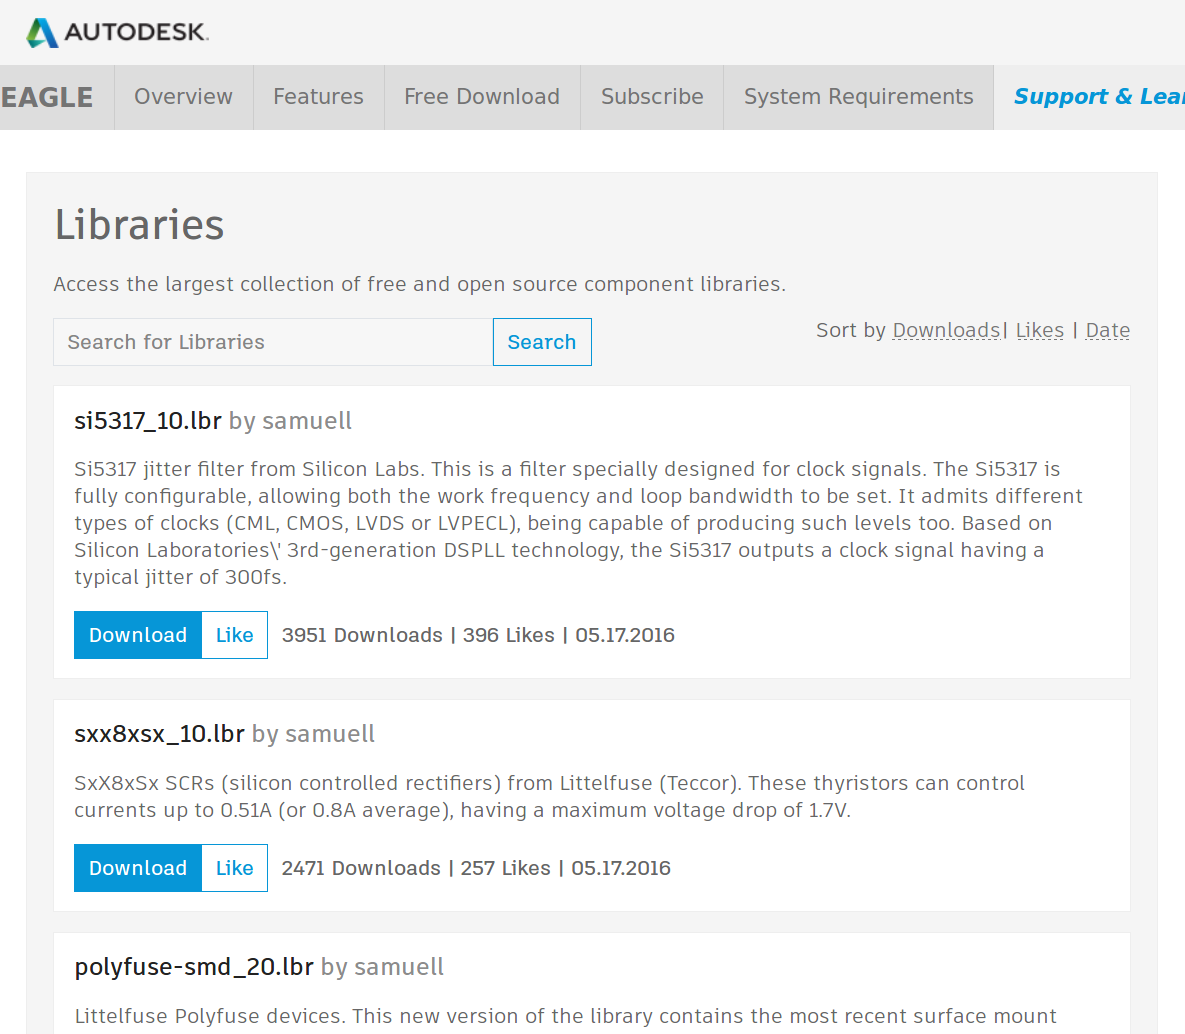
\includegraphics[height=.85\textheight]{images/eagle_libraries_website.png}
      };}
      \onslide<2->{\node (img2) [anchor=north west] at (2cm,-1cm) {
        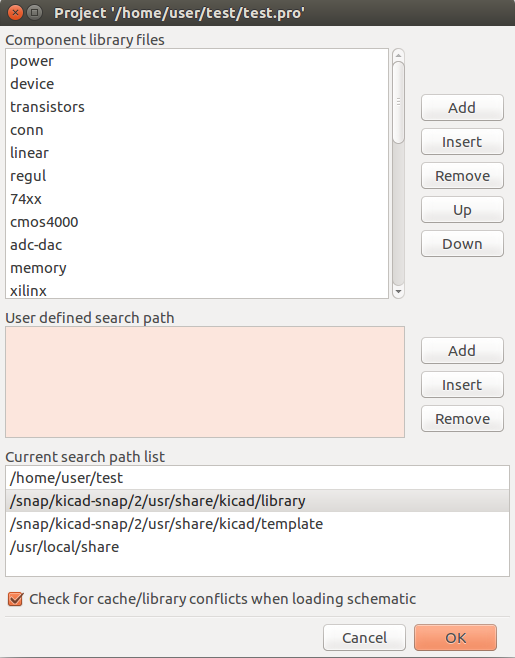
\includegraphics[height=.85\textheight]{images/kicad_component_libraries.png}
      };}
      \onslide<3->{\node (img3) [anchor=north west] at (4cm,-2cm) {
        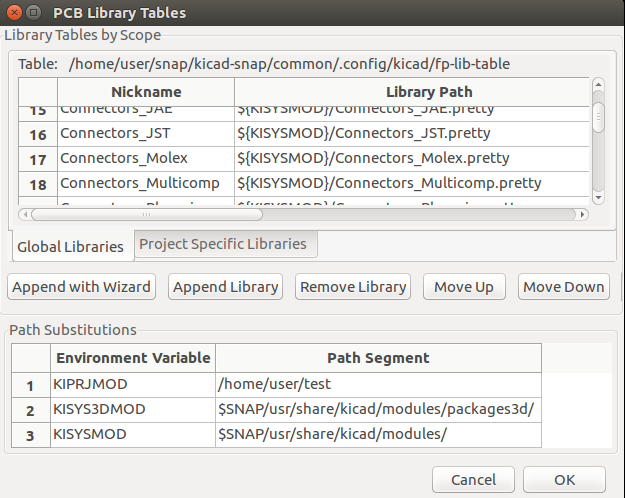
\includegraphics[height=.65\textheight]{images/kicad_library_tables.png}
      };}
      \onslide<4->{\draw (img2.center) node[scale=12] {
        \color{red}{\faQuestion}
      };}
    \end{tikzpicture}
  \end{center}
\end{frame}

\begin{frame}[noframenumbering]{\secname}
  \textbf{Solution}
  \begin{itemize}
    \item Integrated library manager with dependency management
    \item Libraries can contain any entity type (symbols, footprint, ...)
    \item The application handles basically \textbf{everything} for you
  \end{itemize}

  \begin{center}
    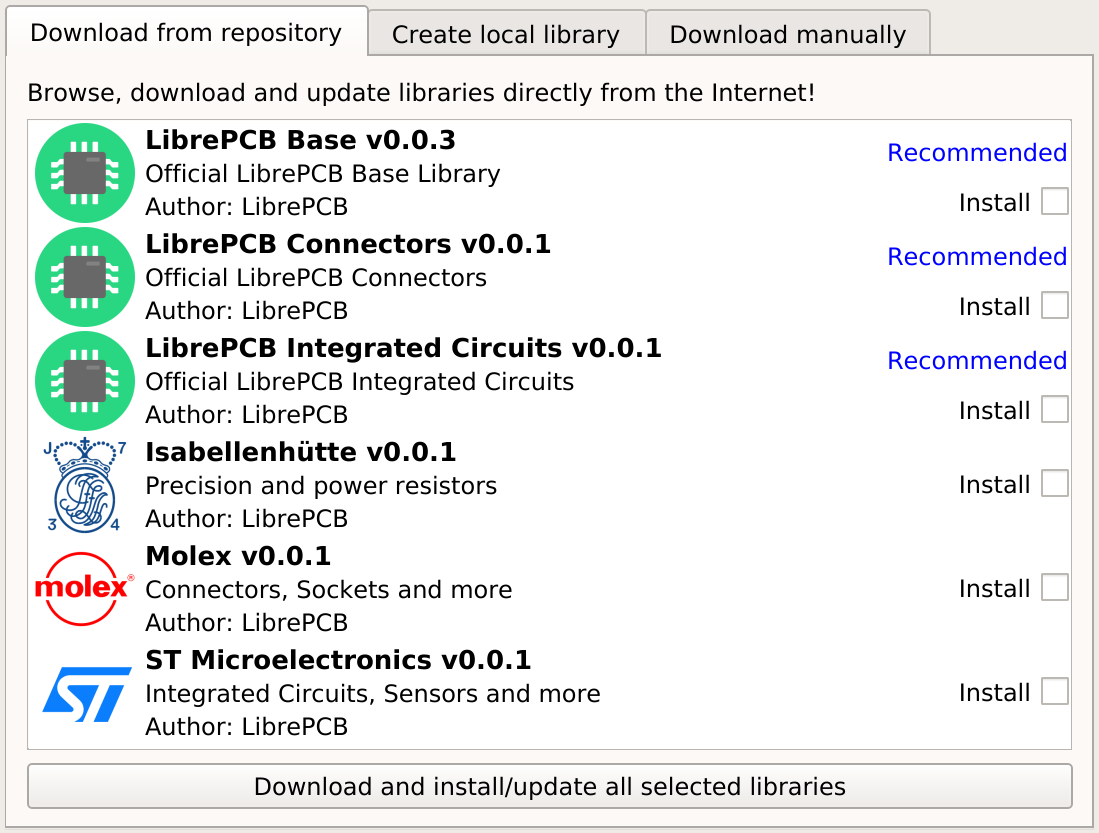
\includegraphics[height=5cm]{images/library_manager.png}
  \end{center}
\end{frame}